\documentclass[compress]{beamer}
\usetheme{sthlm}

%-=-=-=-=-=-=-=-=-=-=-=-=-=-=-=-=-=-=-=-=-=-=-=-=
%        LOADING BEAMER PACKAGES
%-=-=-=-=-=-=-=-=-=-=-=-=-=-=-=-=-=-=-=-=-=-=-=-=

\usepackage{
booktabs,
datetime,
dtk-logos,
graphicx,
multicol,
pgfplots,
ragged2e,
tabularx,
tikz,
wasysym,
multirow,
float,
caption,
subcaption
}

\pgfplotsset{compat=1.8}

\usepackage[utf8]{inputenc}
\usepackage[portuguese]{babel}
\usepackage[T1]{fontenc}
\usepackage{newpxtext,newpxmath}
\usepackage{listings}

\lstset{ %
language=[LaTeX]TeX,
basicstyle=\normalsize\ttfamily,
keywordstyle=,
numbers=left,
numberstyle=\tiny\ttfamily,
stepnumber=1,
showspaces=false,
showstringspaces=false,
showtabs=false,
breaklines=true,
frame=tb,
framerule=0.5pt,
tabsize=4,
framexleftmargin=0.5em,
framexrightmargin=0.5em,
xleftmargin=0.5em,
xrightmargin=0.5em
}



%-=-=-=-=-=-=-=-=-=-=-=-=-=-=-=-=-=-=-=-=-=-=-=-=
%        LOADING TIKZ LIBRARIES
%-=-=-=-=-=-=-=-=-=-=-=-=-=-=-=-=-=-=-=-=-=-=-=-=

\usetikzlibrary{
backgrounds,
mindmap
}

%-=-=-=-=-=-=-=-=-=-=-=-=-=-=-=-=-=-=-=-=-=-=-=-=
%        BEAMER OPTIONS
%-=-=-=-=-=-=-=-=-=-=-=-=-=-=-=-=-=-=-=-=-=-=-=-=

\setbeameroption{show notes}

%-=-=-=-=-=-=-=-=-=-=-=-=-=-=-=-=-=-=-=-=-=-=-=-=
%        BEAMER COMMANDS
%-=-=-=-=-=-=-=-=-=-=-=-=-=-=-=-=-=-=-=-=-=-=-=-=


%-=-=-=-=-=-=-=-=-=-=-=-=-=-=-=-=-=-=-=-=-=-=-=-=
%
%	PRESENTATION INFORMATION
%
%-=-=-=-=-=-=-=-=-=-=-=-=-=-=-=-=-=-=-=-=-=-=-=-=

\title{Comunicação multicast}
\subtitle{DCE540 - Computação Paralela e Distribuída}
%\date{\small{\jobname}}
\author{\texttt{Iago Carvalho}}
\institute{\texttt{Departamento de Ciência da Computação}}

\hypersetup{
pdfauthor = {Iago A. Carvalho},      
pdfsubject = {Computação Paralela e Distribuída},
pdfkeywords = {},  
pdfmoddate= {D:\pdfdate},          
pdfcreator = {WriteLaTeX}
}

\begin{document}

\begin{frame}
\titlepage

\end{frame}

%% --------------------------------------------------------

\begin{frame}{\textit{Multicast} e \textit{broadcast}}

Muitas vezes, as mensagens são enviadas de um componente para outro
\begin{itemize}
    \item Um único remetente
    \item Um único receptor
\end{itemize}

\vspace{0.5cm}

Entretanto, existem tipos de comunicação especiais quando um componente está interessado em enviar mensagens de forma mais ampla
\begin{itemize}
    \item \textit{Broadcast}
    \begin{itemize}
        \item Um para todos
    \end{itemize}
    \item \textit{Multicast}
    \begin{itemize}
        \item Um para muitos
    \end{itemize}
\end{itemize}
\end{frame}

%% --------------------------------------------------------

\begin{frame}{\textit{Broadcast} como forma de \textit{multicast}}

É possível implementar uma operação de \textit{multicast} utilizando \textit{broadcast}

\vspace{0.5cm}

Uma mensagem é transmitida para \textbf{todos} os nós da rede
\begin{itemize}
    \item Mensagem contém um cabeçalho determinando quem é o alvo
    \item O receptor lê o cabeçalho para saber se a mensagem é para ele
\end{itemize}

\vspace{0.5cm}

Implementação é simples e fácil
\begin{itemize}
    \item Entretanto, sobrecarrega a rede com mensagens desnecessárias
\end{itemize}
\end{frame}

%% --------------------------------------------------------

\begin{frame}{\textit{Multicast} utilizando sobreposição de rede}

\textit{Overlay networks} (\textit{Software Defined Networks} (SDN))
\begin{itemize}
    \item Estrutura de rede que é construída sobre outra já existente
    \item Definem caminhos de comunicação entre dois nós da rede
    \item Redes reais ou mapeadas
\end{itemize}

\vspace{1cm}

Existem dois principais tipos de SDNs
\begin{itemize}
    \item Árvores
    \item Redes \textit{mesh}
\end{itemize}

\end{frame}

%% --------------------------------------------------------

\begin{frame}{Árvores}


\centering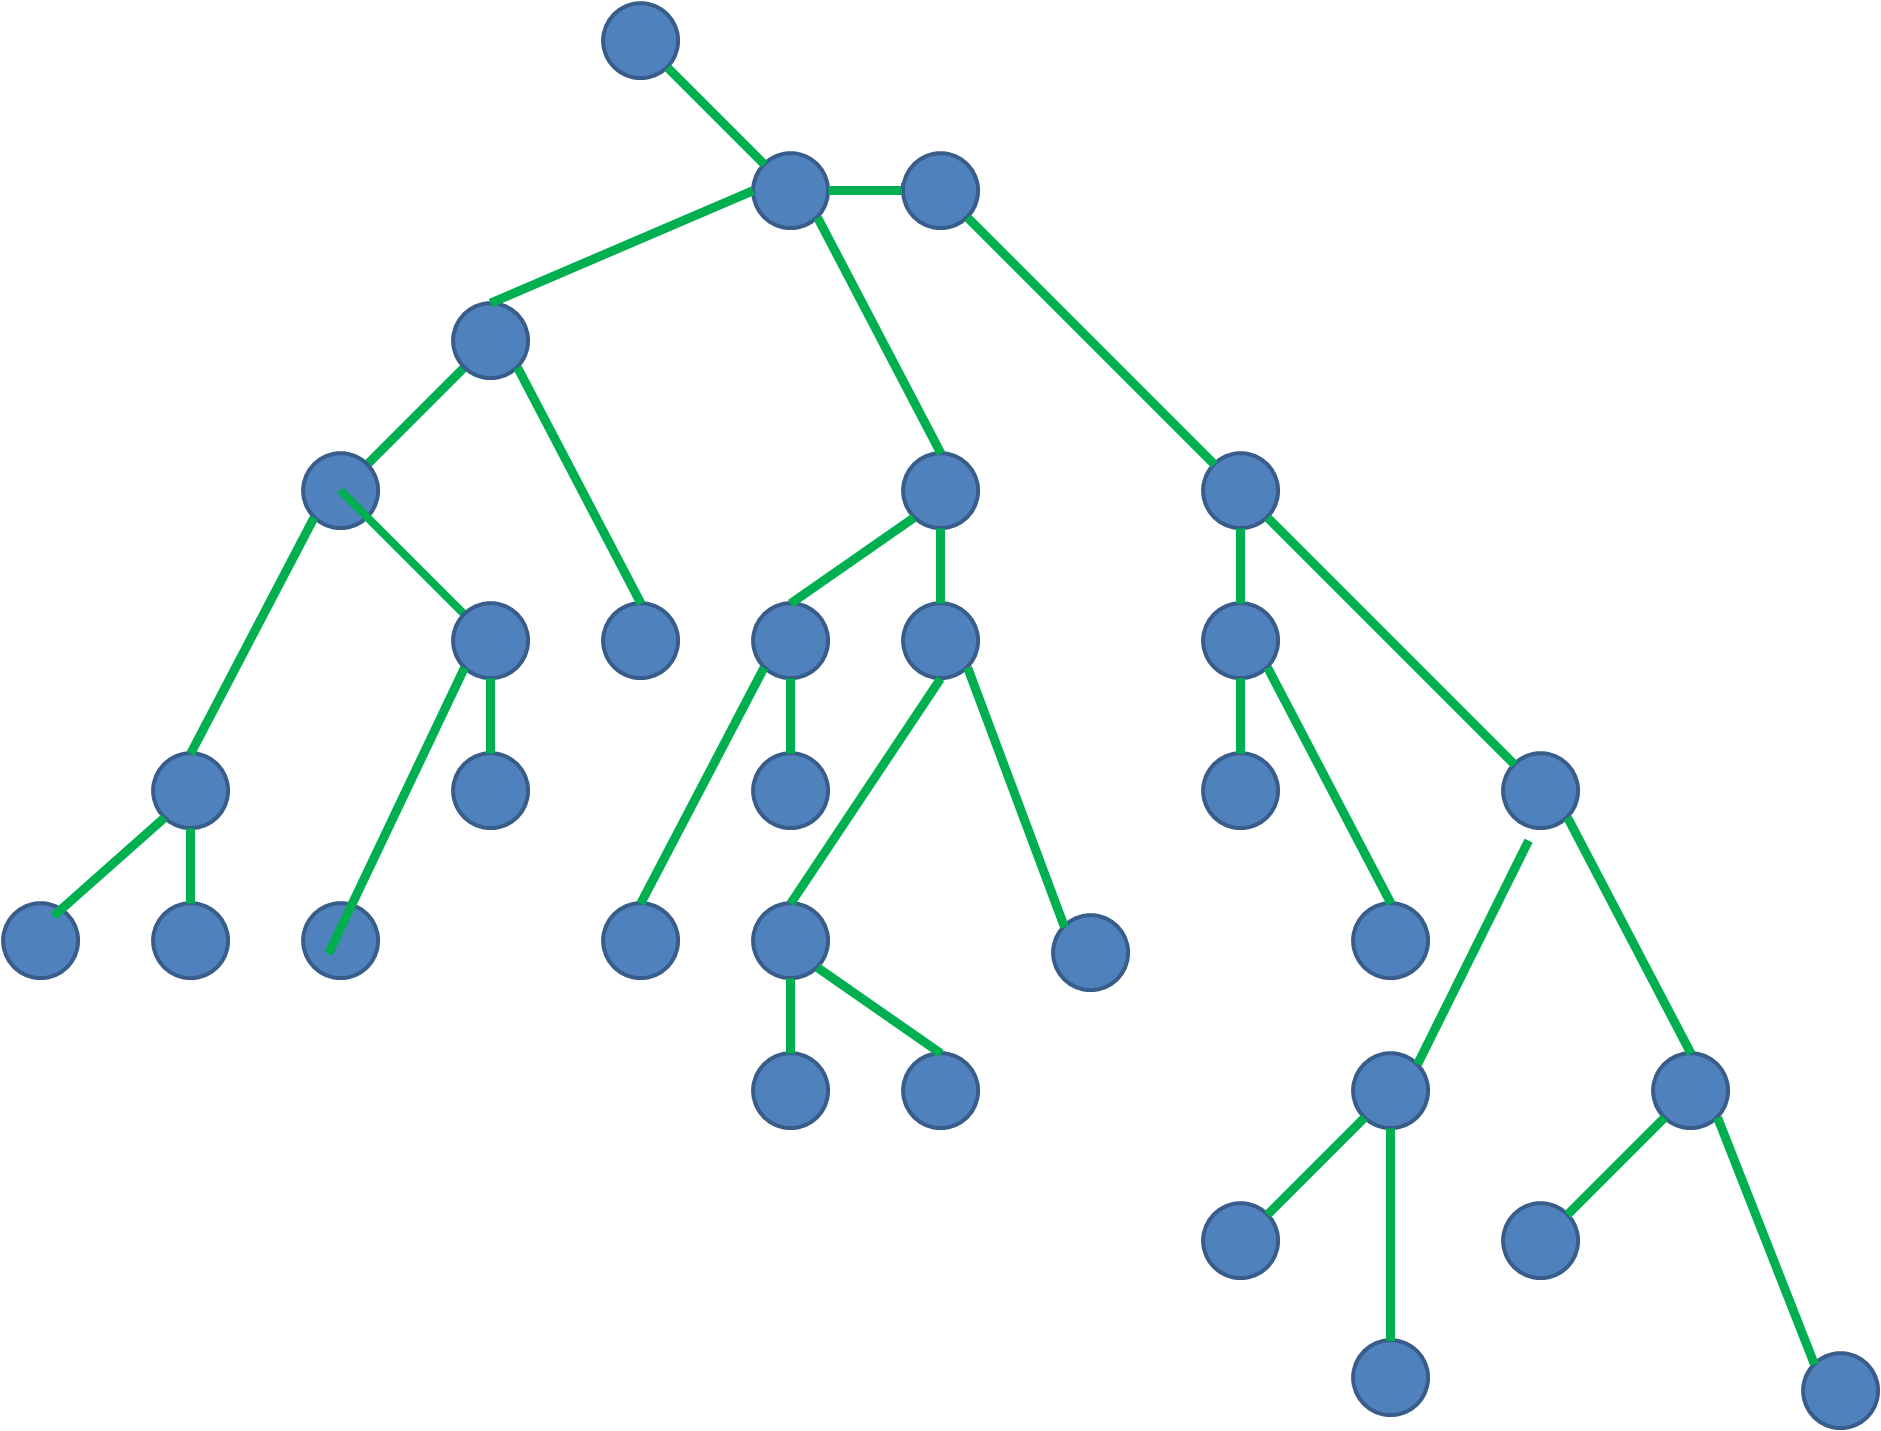
\includegraphics[width=0.9\textwidth]{images/arvore.png}

\end{frame}

%% --------------------------------------------------------

\begin{frame}{Redes \textit{mesh}}


\centering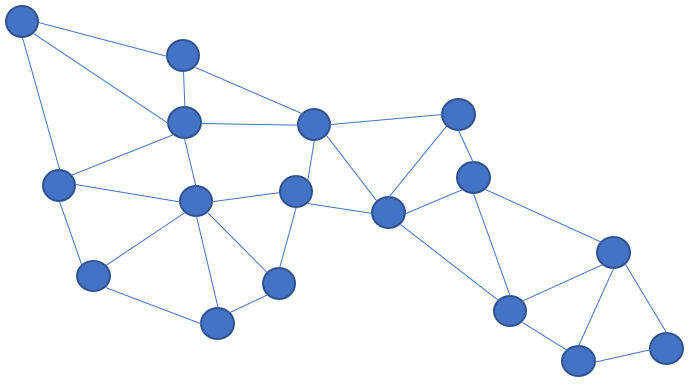
\includegraphics[width=0.9\textwidth]{images/mesh.png}

\end{frame}

%% --------------------------------------------------------

\begin{frame}{\textit{Multicast} por inundação de mensagens}

Uma operação de \textit{broadcast} em uma SDN equivale a realizar \textit{multicast} nos nós participantes daquela SDN

\vspace{0.3cm}

Assim, pode-se inundar a rede com mensagens
\begin{itemize}
    \item Objetivo é obter o broadcast em uma SDN
\end{itemize}

\vspace{0.3cm}

Um nó recebe uma mensagen
\begin{itemize}
    \item Encaminha esta mensagem para todos seus vizinhos (exceto o que enviou a mensagem)
    \item Nó guarda o caminho da mensagem para evitar mensagens duplicadas
    \begin{itemize}
        \item Espaço extra necessário para armazenar o caminho da mensagem
    \end{itemize}
\end{itemize}

\vspace{0.3cm}

Eficiente em árvores, mas ineficiente em redes \textit{mesh}
\end{frame}

%% --------------------------------------------------------

\begin{frame}{\textit{Multicast} por fococas}

Também conhecido como modelo epidêmico

\vspace{0.3cm}

Modelo descentralizado para realizar \textit{multicast}

\vspace{0.3cm}

Nós são separados em três categorias
\begin{itemize}
    \item Infectado: nós que possuem a mensagem e querem repassa-las
    \item Sucetível: nós que ainda não possuem a mensagem
    \item Removido: nós que já possuem a mensagem mas não desejam repassa-las
\end{itemize}

\vspace{0.3cm}

Neste modelo, o objetivo é que o maior número de nós sejam infectados
\begin{itemize}
    \item Um nó sucetível pode ser infectado caso o segundo entre em contato com o primeiro
\end{itemize}
\end{frame}

\end{document}
